\documentclass{beamer}
\usetheme{metropolis}
\usepackage{graphicx}
\usepackage{amsmath}
\usepackage{url}

\def\rcurs{{\mbox{$\resizebox{.16in}{.08in}{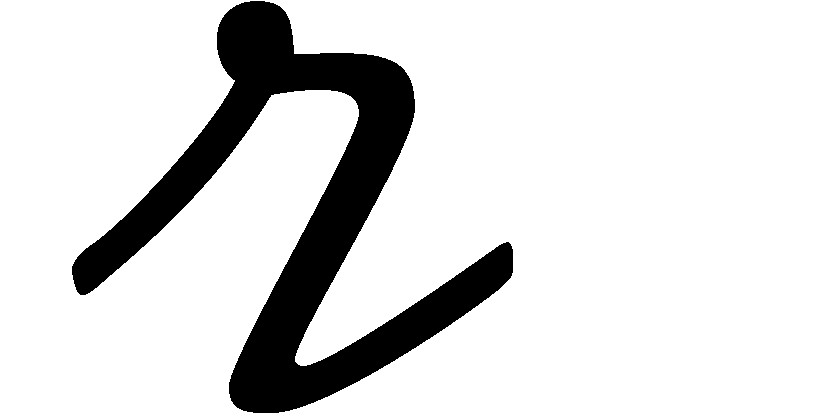
\includegraphics{ScriptR}}$}}}
\def\brcurs{{\mbox{$\resizebox{.16in}{.08in}{
\includegraphics{BoldR}}$}}}
\def\hrcurs{{\mbox{$\hat \brcurs$}}}

\title{Electromagnetc Theory: PHYS330}
\author{Jordan Hanson}
\institute{Whittier College Department of Physics and Astronomy}

\begin{document}
\maketitle

\section{Summary}

\begin{frame}{Week 6 Summary}
\begin{enumerate}
\item Current and Newton's Law
\item Flux rule from Lorentz force
\item Faraday's Law: Inspired by Symmetry
\begin{itemize}
\item Induced E-fields
\item Quasi-static behavior
\end{itemize}
\item Inductors and analog filtering (special topic)
\end{enumerate}
\end{frame}

\section{Current and Newton's Law}

\begin{frame}{Current and Newton's Law}
Why does current move at a constant velocity, if it is driven by an electric field?
\begin{equation}
\vec{J} = \sigma (\vec{E} + \vec{v} \times \vec{B} ) = \sigma \vec{E}
\end{equation}
This formula governs the current density as a function of force per unit charge, and it assumes small drift velocities so that the magnetic contributions are zero. \\ \vspace{0.5cm}
\textit{What is the acceleration of an electron in the middle of a parallel plate capacitor with empty space in the middle? } Let the charge density be 1 $\mu$ C per cm$^2$.  The mass of an electron is $9.1\times 10^{-31}$ kg, and $\epsilon_0 = 8.85 \times 10^{-12}$ F/m.
\end{frame}

\begin{frame}{Current and Newton's Law}
Why does current move at a constant velocity, if it is driven by an electric field?
\begin{equation}
\vec{J} = \sigma (\vec{E} + \vec{v} \times \vec{B} ) = \sigma \vec{E}
\end{equation}
This formula governs the current density as a function of force per unit charge, and it assumes small drift velocities so that the magnetic contributions are zero. \\ \vspace{0.5cm}
\textit{What is the acceleration of a charge flowing in a conductor that connects the parallel plates of the capacitor?} Let the charge density be 1 $\mu$ C per cm$^2$.  The mass of an electron is $9.1\times 10^{-31}$ kg, and $\epsilon_0 = 8.85 \times 10^{-12}$ F/m.  Let the total effective resitance be 1 $\Omega$.
\end{frame}

\begin{frame}{Current and Newton's Law}
\begin{figure}
\centering
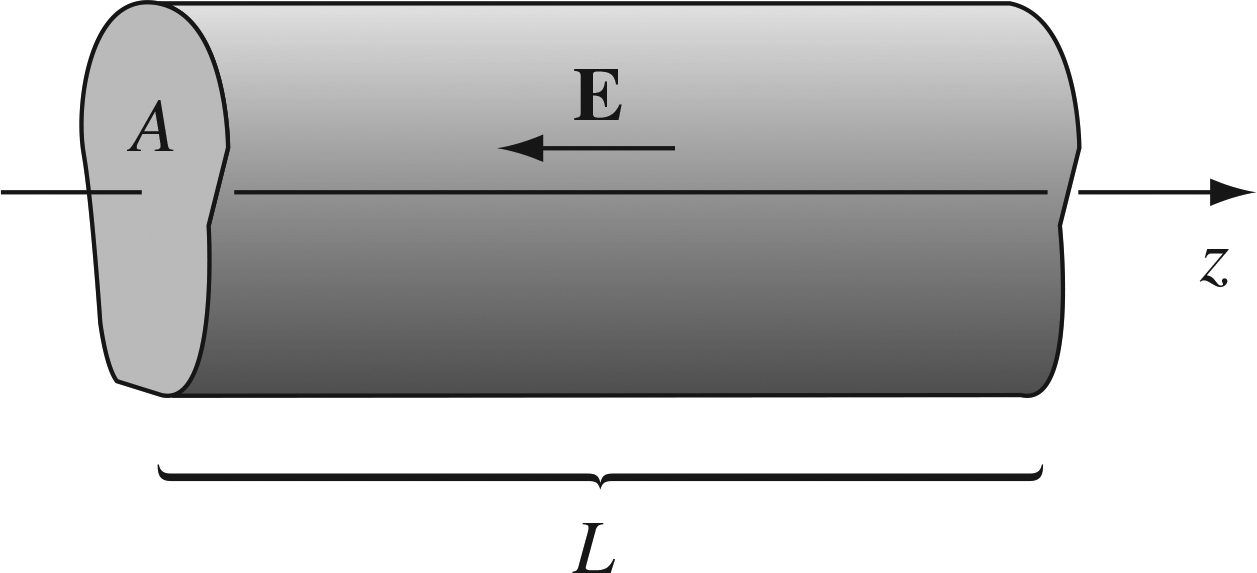
\includegraphics[width=5cm]{figures/7_1.jpg}
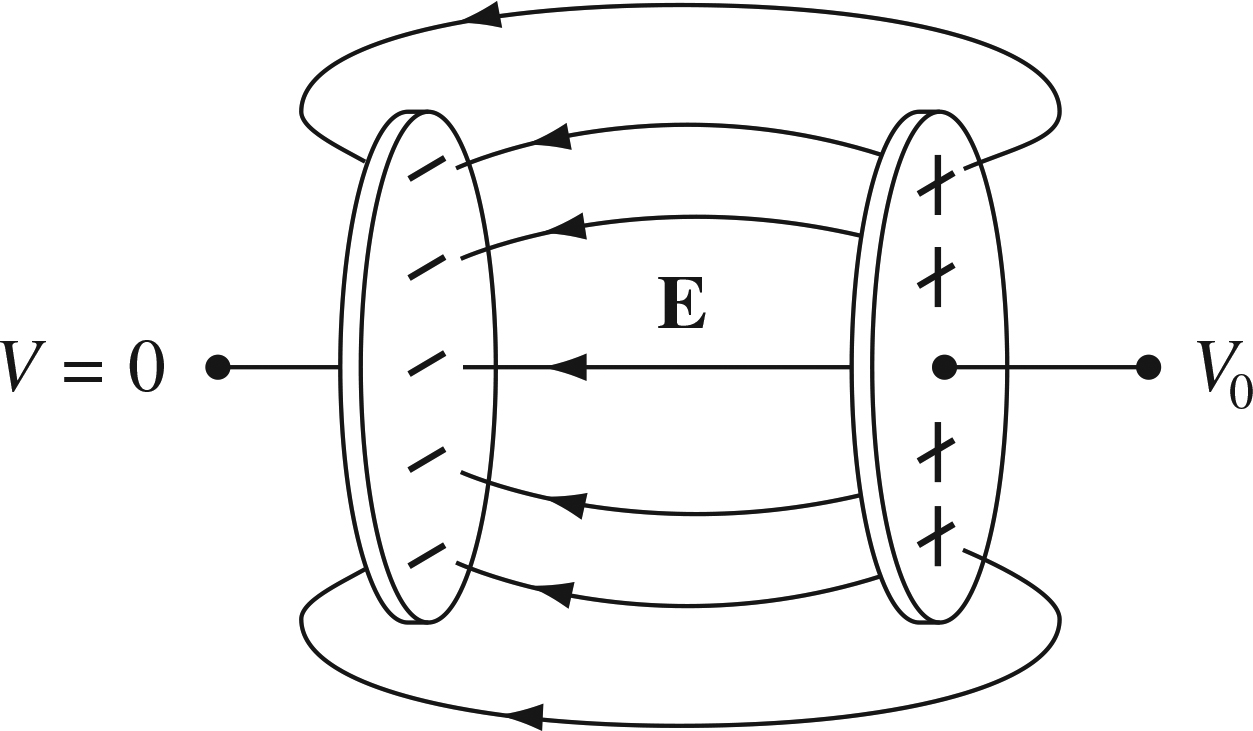
\includegraphics[width=5cm]{figures/7_3.jpg}
\caption{\label{fig:cond1} (Left) A conductor. (Right) A capacitor with the same geometry.}
\end{figure}
\begin{itemize}
\item Convince yourself that if the potential difference between the left and right sides of the conductor (left) is $V_0 - 0 = V_0$, that $V(z) = (V_0/L) z$.
\item The E-field is therefore $\vec{E} = - V_0/L \hat{z}$, but the current does not accelerate.
\end{itemize}
\end{frame}

\section{Motional EMF Problems: Flux Rule from the Lorentz Force}

\begin{frame}{Flux Rule from Lorentz Force}
\begin{figure}
\centering
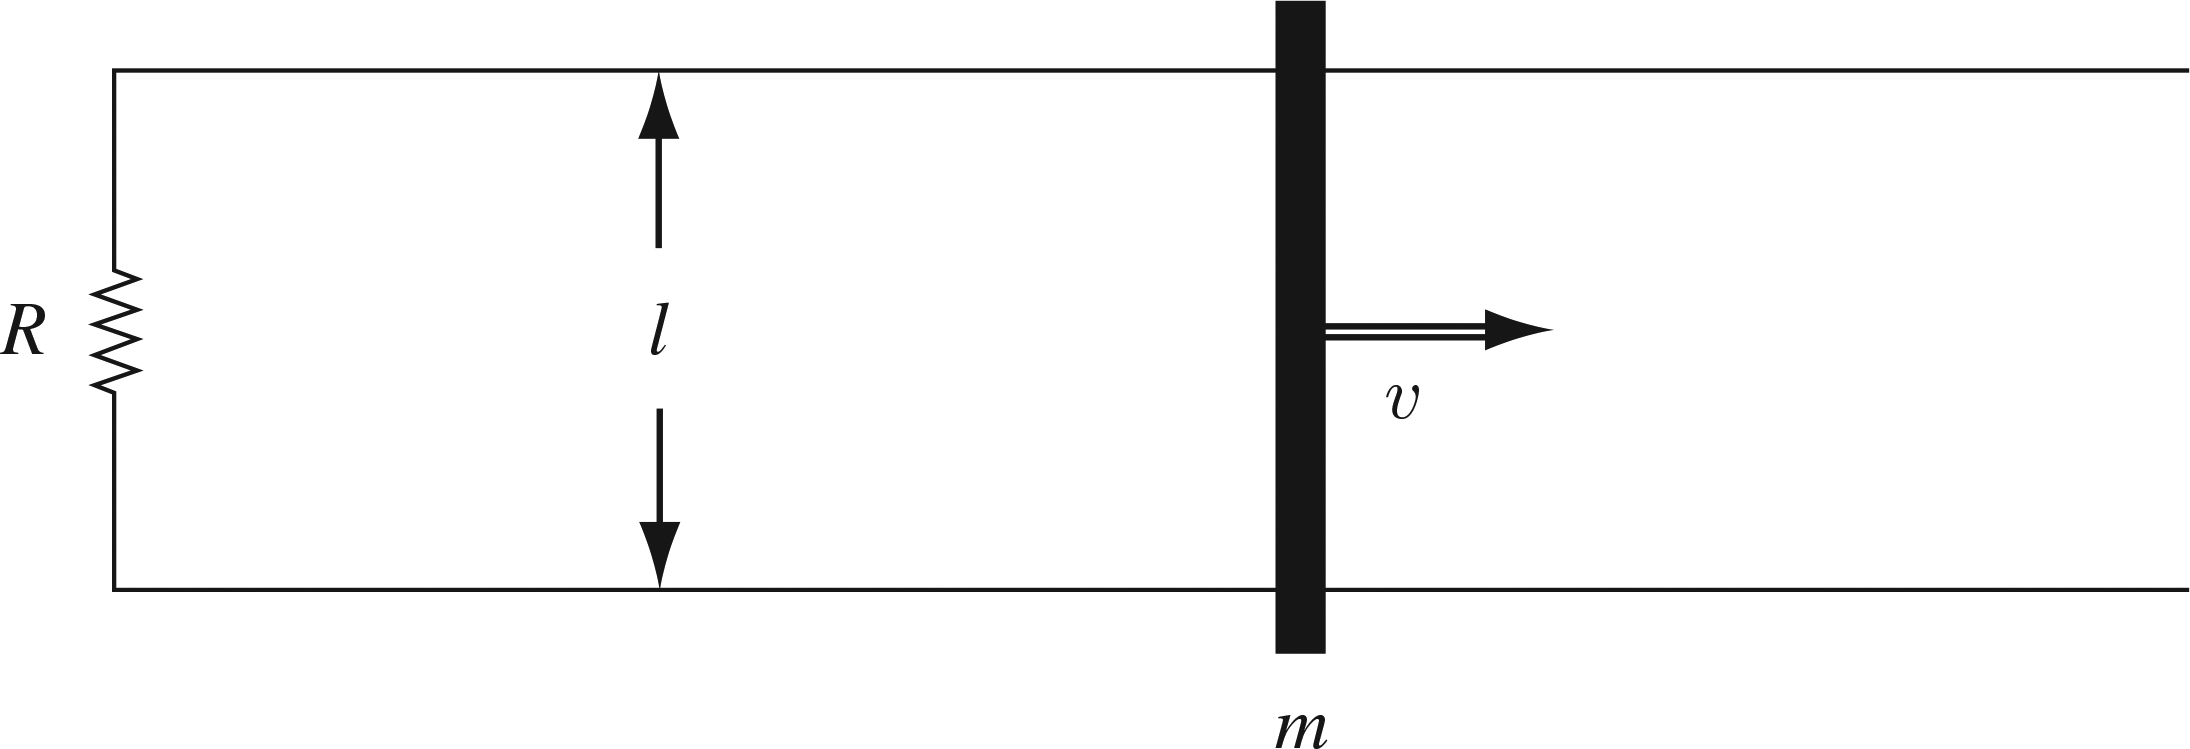
\includegraphics[width=7cm]{figures/7_17.jpg} \\
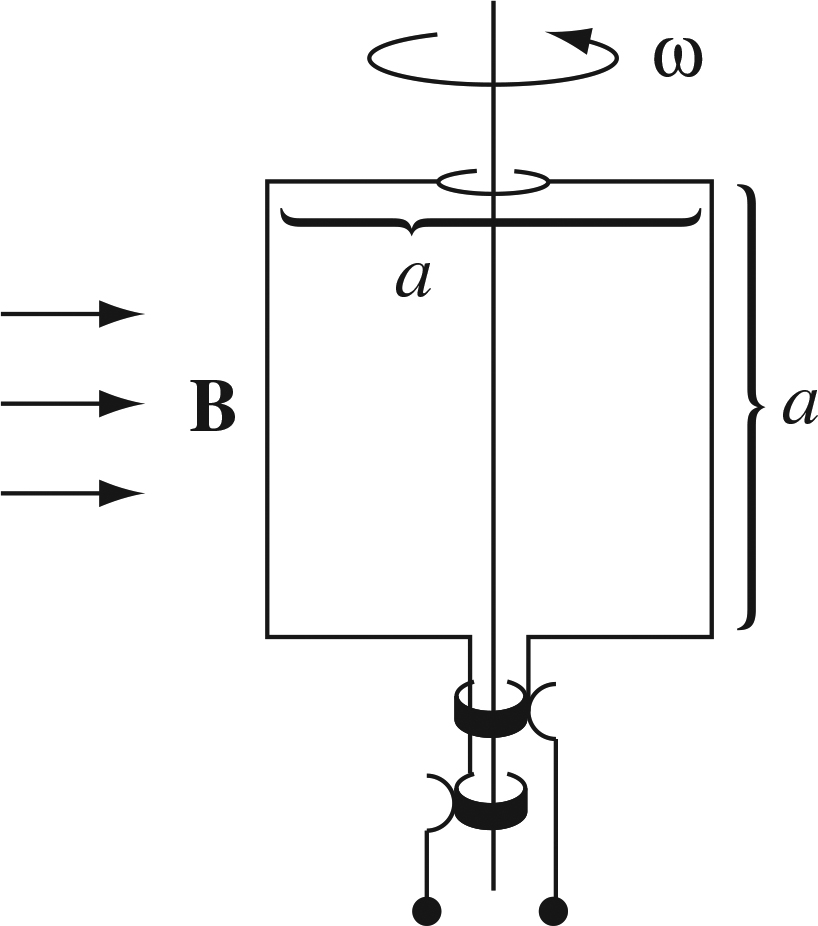
\includegraphics[width=3.0cm]{figures/7_19.jpg}
\caption{\label{fig:gen} Motional emf problems resulting from the Lorentz force, solvable by the flux rule. (Top) Frictionless rails problem ... rail guns.  (Bottom): the AC generator.}
\end{figure}
\end{frame}

\section{Faraday's Law: Inspired by Symmetry}

\begin{frame}{Faraday's Law}
\alert{\textbf{In words:}} E-fields (via currents) generate B-fields.  Changing B-fields induce E-fields (in loops). 
In differential form:
\begin{equation}
\boxed{
\nabla \times \vec{E} = -\frac{\partial \vec{B}}{\partial t}
}
\end{equation}
In integral form (via Stoke's Theorem):
\begin{equation}
\boxed{
\oint \vec{E} \cdot d\vec{l} = - \frac{\partial}{\partial t} \int \vec{B} \cdot d\vec{a}
}
\end{equation}
\end{frame}

\begin{frame}{Faraday's Law}
\begin{figure}
\centering
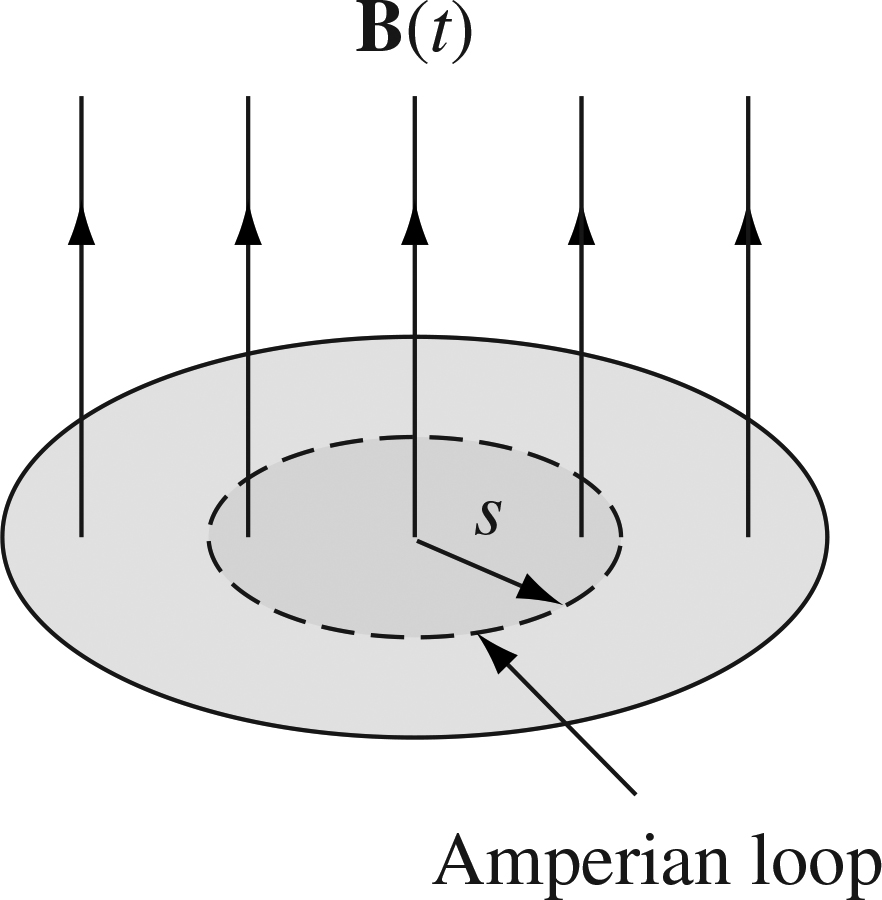
\includegraphics[width=4cm]{figures/7_25.jpg} \\
\caption{\label{fig:far1} Cylindrical symmetry and the use of Faraday's Law to obtain emf.}
\end{figure}
\begin{itemize}
\item What is the magnitude and shape of the $\vec{E}$-field a distance $s$ from the origin?
\item What is the current $I$ in a loop of wire at the same radius?
\end{itemize}
\end{frame}

\begin{frame}{Faraday's Law}
\begin{figure}
\centering
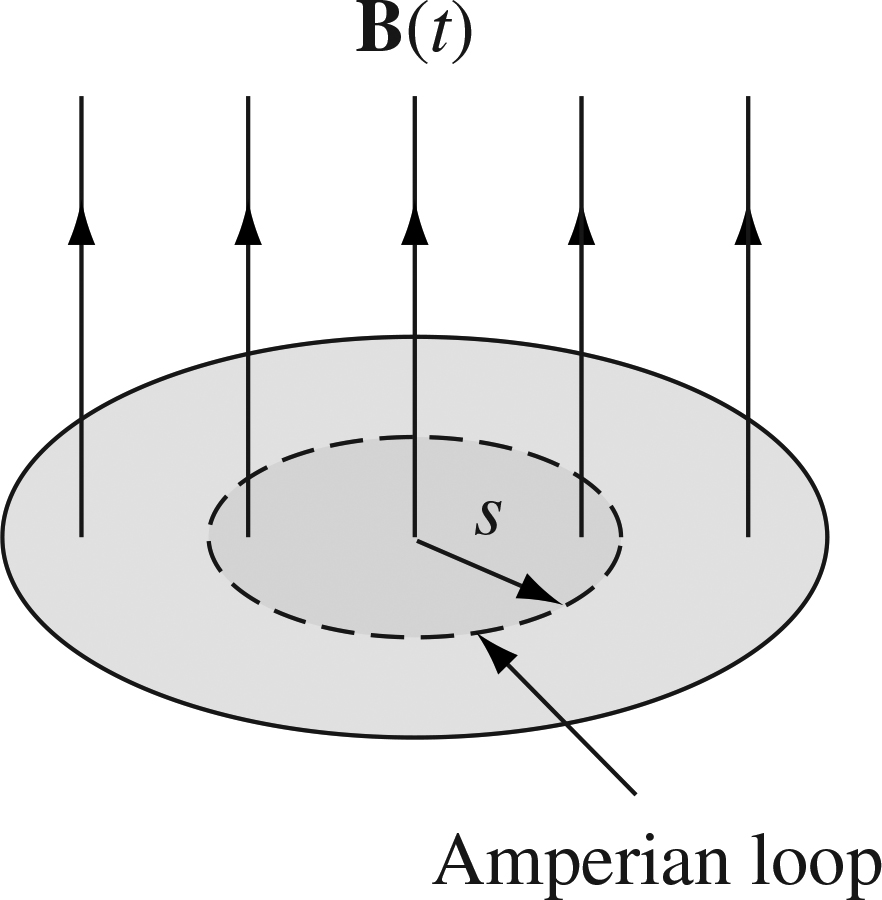
\includegraphics[width=4cm]{figures/7_25.jpg} \\
\caption{\label{fig:far1} Cylindrical symmetry and the use of Faraday's Law to obtain emf.}
\end{figure}
\begin{itemize}
\item What is the acceleration of a point charge located a distance $s$ from the origin?
\end{itemize}
\end{frame}

\begin{frame}{Faraday's Law}
\textbf{Exercise 7.13:} A square loop of wire, with sides of length a, lies in the first quadrant of the xy-plane, with one corner at the origin.  In this region, there is a nonuniform time-dependent magnetic field $\vec{B}(y,t) = k y^3 t^2 \hat{z}$ (where $k$ is constant).  Find the emf induced in the loop. \\ \vspace{6cm}
\end{frame}

\begin{frame}{Faraday's Law}
\textbf{Quasi-static behavior:}  $I(t)$ varies slowly enough to use the techniques of \textit{magnetostatics} to predict $\vec{B}(t)$\footnote{Imagine the changing B-field changes so fast that the speed of light comes into play.  For example, when the observer is so far away that the field's ``wave'' takes time to reach the observer.}. \\ \vspace{0.25cm}
An infinitely long wire caries a current $I(t)$. Determine the induced E-field as a function of distance $s$ from the wire. (Find the direction first).
\begin{figure}
\centering
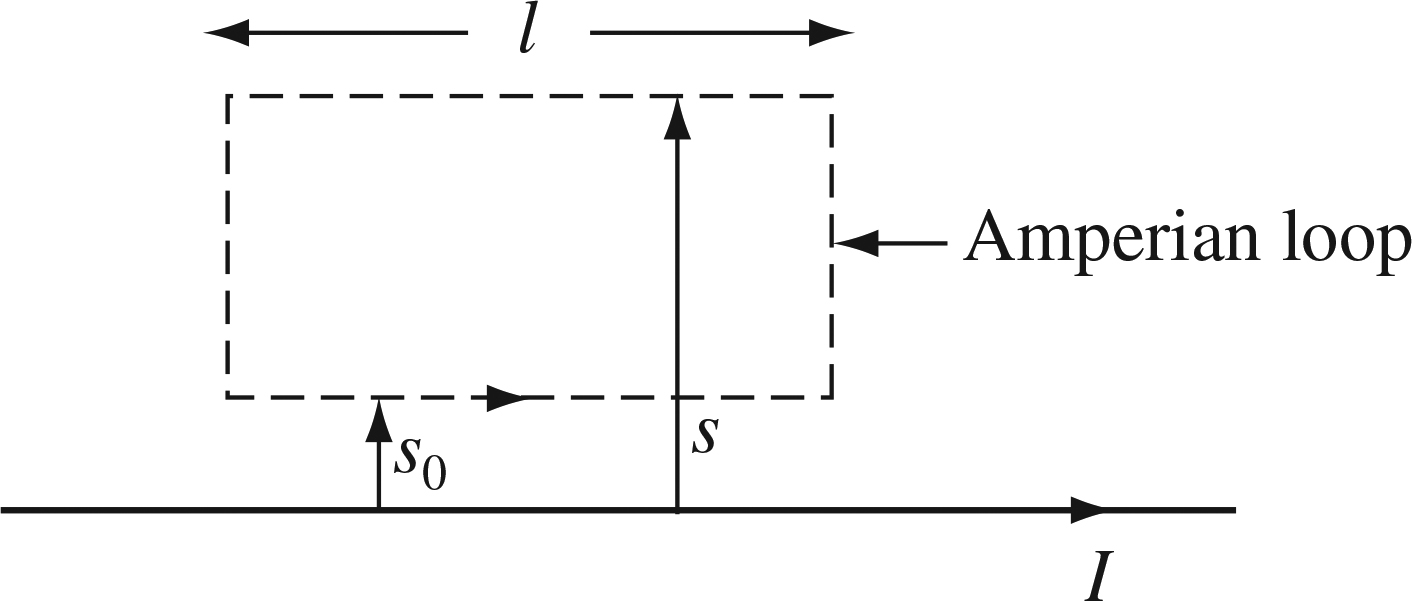
\includegraphics[width=5cm]{figures/7_27.jpg} \\
\caption{\label{fig:far2} Obtaining the E-field generated by a long wire.}
\end{figure}
\end{frame}

\begin{frame}{Faraday's Law}
A long solenoid of radius $a$, carrying $n$ turns per unit length, is looped by a wire with resistance $R$.
\begin{itemize}
\item (a) If the current in the solenoid is increasing at a constant rate $dI/dt = k$, what current flows and in what direction?
\item (b) If the current is constant but the solenoid is removed to the left, what total charge passes through the resistor?
\end{itemize}
\begin{figure}
\centering
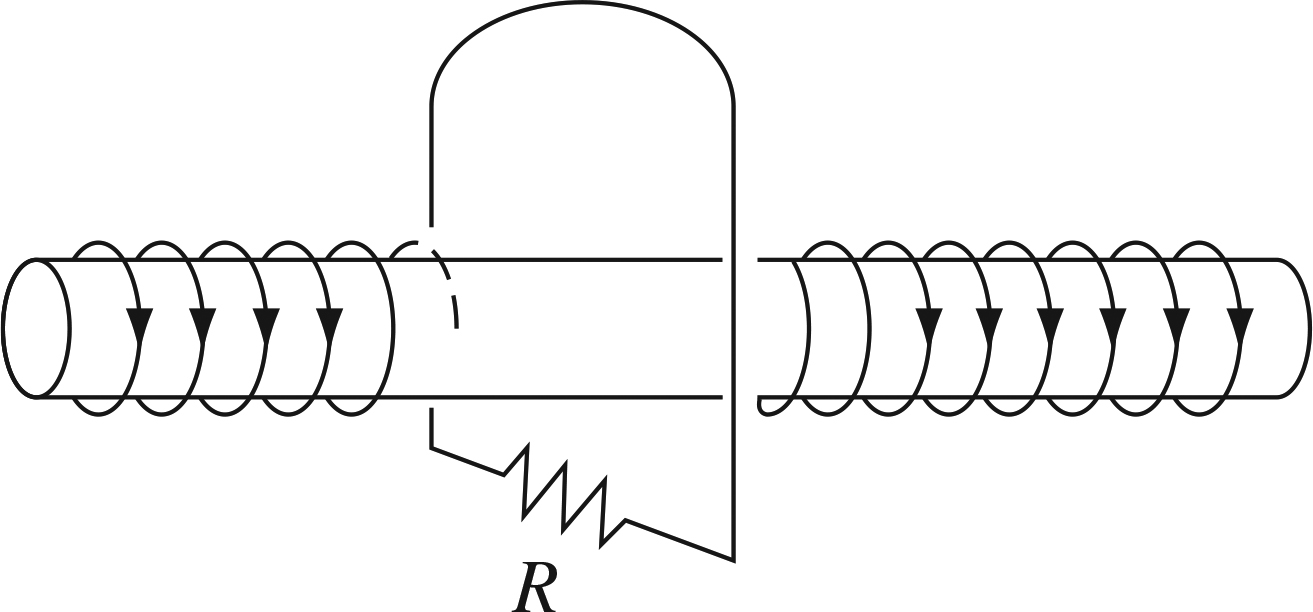
\includegraphics[width=5cm]{figures/7_28.jpg} \\
\caption{\label{fig:far3} Obtaining the E-field generated by a long solenoid.}
\end{figure}
\end{frame}

\section{Special Topic: Inductors and Analog Filtering of Voltage Signals}

\begin{frame}[fragile]{Inductors and Analog Filtering of Voltage Signals}
\small
\textit{\alert{There is so much more here, especially in electrical engineering!}} Remember the AC-circuit elements from before? We can now understand the origin of the impedences!  Recall that Ohm's law is $v = i R$ in \textit{both the time-domain and the frequency domain.}
\begin{itemize}
\item (The resistor is trivial). if $R$ is a constant, then the Fourier transform of a constant is a constant.  Thus, $Z_R = R$.
\item Definition of capacitance: $Q = CV$.  Take the derivative of both sides and then take the Fourier transform of both sides, compare to Ohm's law.
\item Definition of inductance: $L = \phi_B/i$, the ratio of magnetic flux to current. Solve for the flux, then take the negative derivative of both sides.  Use Lenz's law $v = -d\phi_B/dt$.  Now take the Fourier transform of both sides and rearrange.  Compare to Ohm's law.
\end{itemize}
\end{frame}

\begin{frame}{Inductors and Analog Filtering of Voltage Signals}
\small
\begin{equation}
\mathcal{F}(f(t)) = \tilde{F}(\omega) = \int_{-\infty}^{\infty} f(t) e^{-j\omega t} dt
\label{eq:eq1}
\end{equation}
In Eq. \ref{eq:eq1}, $\omega$ is the angular frequency, measured in radians per unit time.  Let $f(t) = g'(t)$.  Substituting into Eq. \ref{eq:eq1}, and integrating by parts, we have
\begin{equation}
\tilde{F}(\omega) = g(t) e^{-j\omega t} |_{-\infty}^{\infty} + j\omega \int_{\infty}^{-\infty} g(t)  e^{-j\omega t} dt
\label{eq:eq2}
\end{equation}
For physical signals that represent finite energy, $\lim_{|t|\rightarrow\infty} g(t) = 0$.  This requirement simplifies Eq. \ref{eq:eq2} by making the first term on the right-hand side vanish.
\end{frame}

\begin{frame}{Inductors and Analog Filtering of Voltage Signals}
\small
\begin{equation}
\tilde{F}(\omega) = j\omega \int_{\infty}^{-\infty} g(t)  e^{-j\omega t} dt = j\omega\mathcal{F}(g(t))
\end{equation}
The result may be summarized:
\begin{equation}
\boxed{
\mathcal{F}(g'(t)) = j\omega\mathcal{F}(g(t))
}
\end{equation}
\end{frame}

\begin{frame}{Inductors and Analog Filtering of Voltage Signals}
\textbf{Example: The response of a circuit with inductors, a capacitor and a resistor.}
\begin{figure}
\centering
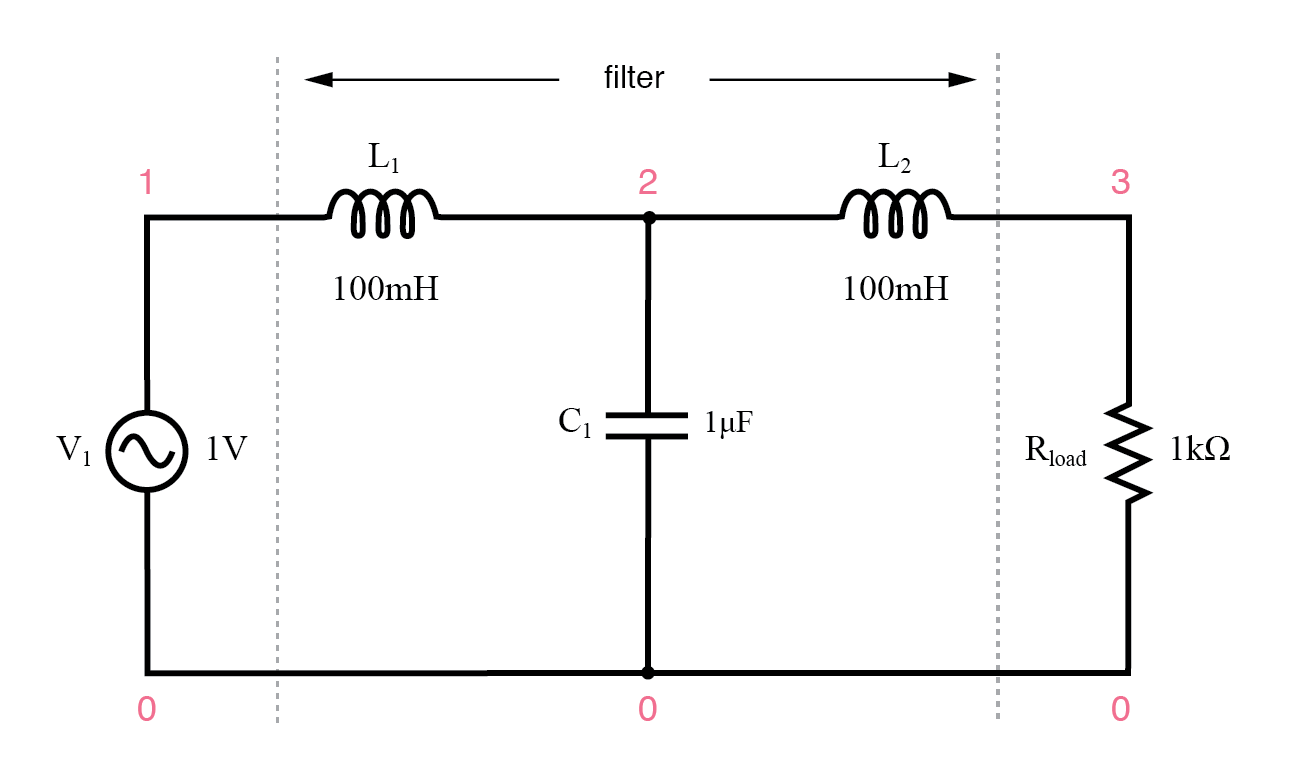
\includegraphics[width=7cm]{figures/filter.png}
\caption{\label{fig:filter} What is the response of the circuit?  That is, amplitude as a function of frequency?}
\end{figure}
\end{frame}

\section{Conclusion}

\begin{frame}{Week 6 Summary}
\begin{enumerate}
\item Current and Newton's Law
\item Flux rule from Lorentz force
\item Faraday's Law: Inspired by Symmetry
\begin{itemize}
\item Induced E-fields
\item Quasi-static behavior
\end{itemize}
\item Inductors and analog filtering (special topic)
\end{enumerate}
\end{frame}

\end{document}
